
\documentclass[a4paper,11pt]{article}
\usepackage[a4paper, margin=8em]{geometry}

% usa i pacchetti per la scrittura in italiano
\usepackage[french,italian]{babel}
\usepackage[T1]{fontenc}
\usepackage[utf8]{inputenc}
\frenchspacing 

% usa i pacchetti per la formattazione matematica
\usepackage{amsmath, amssymb, amsthm, amsfonts}

% usa altri pacchetti
\usepackage{gensymb}
\usepackage{hyperref}
\usepackage{standalone}

% imposta il titolo
\title{Appunti Calcolo Numerico}
\author{Luca Seggiani}
\date{2025}

% disegni
\usepackage{pgfplots}
\pgfplotsset{width=10cm,compat=1.9}

% imposta lo stile
% usa helvetica
\usepackage[scaled]{helvet}
% usa palatino
\usepackage{palatino}
% usa un font monospazio guardabile
\usepackage{lmodern}

% tikz in sans
\tikzset{every picture/.style={/utils/exec={\sffamily}}}

\renewcommand{\rmdefault}{ppl}
\renewcommand{\sfdefault}{phv}
\renewcommand{\ttdefault}{lmtt}

% circuiti
\usepackage{circuitikz}
\usetikzlibrary{babel}

% disponi il titolo
\makeatletter
\renewcommand{\maketitle} {
	\begin{center} 
		\begin{minipage}[t]{.8\textwidth}
			\textsf{\huge\bfseries \@title} 
		\end{minipage}%
		\begin{minipage}[t]{.2\textwidth}
			\raggedleft \vspace{-1.65em}
			\textsf{\small \@author} \vfill
			\textsf{\small \@date}
		\end{minipage}
		\par
	\end{center}

	\thispagestyle{empty}
	\pagestyle{fancy}
}
\makeatother

% disponi teoremi
\usepackage{tcolorbox}
\newtcolorbox[auto counter, number within=section]{theorem}[2][]{%
	colback=blue!10, 
	colframe=blue!40!black, 
	sharp corners=northwest,
	fonttitle=\sffamily\bfseries, 
	title=Teorema~\thetcbcounter: #2, 
	#1
}

% disponi definizioni
\newtcolorbox[auto counter, number within=section]{definition}[2][]{%
	colback=red!10,
	colframe=red!40!black,
	sharp corners=northwest,
	fonttitle=\sffamily\bfseries,
	title=Definizione~\thetcbcounter: #2,
	#1
}

% disponi problemi
\newtcolorbox[auto counter, number within=section]{problem}[2][]{%
	colback=green!10,
	colframe=green!40!black,
	sharp corners=northwest,
	fonttitle=\sffamily\bfseries,
	title=Problema~\thetcbcounter: #2,
	#1
}

% disponi codice
\usepackage{listings}
\usepackage[table]{xcolor}

\definecolor{codegreen}{rgb}{0,0.6,0}
\definecolor{codegray}{rgb}{0.5,0.5,0.5}
\definecolor{codepurple}{rgb}{0.58,0,0.82}
\definecolor{backcolour}{rgb}{0.95,0.95,0.92}

\lstdefinestyle{codestyle}{
		backgroundcolor=\color{black!5}, 
		commentstyle=\color{codegreen},
		keywordstyle=\bfseries\color{magenta},
		numberstyle=\sffamily\tiny\color{black!60},
		stringstyle=\color{green!50!black},
		basicstyle=\ttfamily\footnotesize,
		breakatwhitespace=false,         
		breaklines=true,                 
		captionpos=b,                    
		keepspaces=true,                 
		numbers=left,                    
		numbersep=5pt,                  
		showspaces=false,                
		showstringspaces=false,
		showtabs=false,                  
		tabsize=2
}

\lstdefinestyle{shellstyle}{
		backgroundcolor=\color{black!5}, 
		basicstyle=\ttfamily\footnotesize\color{black}, 
		commentstyle=\color{black}, 
		keywordstyle=\color{black},
		numberstyle=\color{black!5},
		stringstyle=\color{black}, 
		showspaces=false,
		showstringspaces=false, 
		showtabs=false, 
		tabsize=2, 
		numbers=none, 
		breaklines=true
}

\lstdefinelanguage{javascript}{
	keywords={typeof, new, true, false, catch, function, return, null, catch, switch, var, if, in, while, do, else, case, break},
	keywordstyle=\color{blue}\bfseries,
	ndkeywords={class, export, boolean, throw, implements, import, this},
	ndkeywordstyle=\color{darkgray}\bfseries,
	identifierstyle=\color{black},
	sensitive=false,
	comment=[l]{//},
	morecomment=[s]{/*}{*/},
	commentstyle=\color{purple}\ttfamily,
	stringstyle=\color{red}\ttfamily,
	morestring=[b]',
	morestring=[b]"
}

% disponi sezioni
\usepackage{titlesec}

\titleformat{\section}
	{\sffamily\Large\bfseries} 
	{\thesection}{1em}{} 
\titleformat{\subsection}
	{\sffamily\large\bfseries}   
	{\thesubsection}{1em}{} 
\titleformat{\subsubsection}
	{\sffamily\normalsize\bfseries} 
	{\thesubsubsection}{1em}{}

% disponi alberi
\usepackage{forest}

\forestset{
	rectstyle/.style={
		for tree={rectangle,draw,font=\large\sffamily}
	},
	roundstyle/.style={
		for tree={circle,draw,font=\large}
	}
}

% disponi algoritmi
\usepackage{algorithm}
\usepackage{algorithmic}
\makeatletter
\renewcommand{\ALG@name}{Algoritmo}
\makeatother

% disponi numeri di pagina
\usepackage{fancyhdr}
\fancyhf{} 
\fancyfoot[L]{\sffamily{\thepage}}

\makeatletter
\fancyhead[L]{\raisebox{1ex}[0pt][0pt]{\sffamily{\@title \ \@date}}} 
\fancyhead[R]{\raisebox{1ex}[0pt][0pt]{\sffamily{\@author}}}
\makeatother

\begin{document}

% sezione (data)
\section{Lezione del 21-03-25}

% stili pagina
\thispagestyle{empty}
\pagestyle{fancy}

\lstset{style=codestyle, language=matlab}

% testo
\subsection{Valutazione della riducibilità}
Riprendiamo il discorso delle matrici riducibili, soffermandoci sul come capire quando una matrice è riducibile, e come ricavare, in caso affermativo, la marice di permutazione $\Pi$ corrispondente.

Vale il seguente risultato (abbastanza banale guardando a quanto detto riguardo alle matrici irriducibili):
\begin{theorem}{Caratterizzazione di matrice riducibile}
	Una matrice $A$ è riducibile quando non è irriducibile, cioè quando il suo grafo associato $G(A)$ non è fortemente connesso.
\end{theorem}

La dimostrazione avviene osservando innanzitutto questo \textbf{lemma}: se esiste una certa permutazione $\pi$ degli elementi in riga, si può ricavare una matrice di permutazione $\Pi$ e definire la matrice:
$$
A' = \Pi A \Pi^T
$$
Avremo allora che il grafo associato ad $A'$ sarà lo stesso associato a $\Pi A \Pi^T$, solamente cambiando i nomi dei vertici, cioè:
$$
G(A) \text{ fortemente connesso} \ \Leftrightarrow \  G(A') \text{ fortemente connesso }
$$

La \textbf{dimostrazione} vera e propria dovrà quindi affermaredovrà quindi affermare che se una matrice è rducibile, allora il suo grafo non è fortemente connesso, cioè:
$$
A \text{ riducibile} \ \Leftrightarrow \  G(A) \text{ non fortemente connesso }
$$

\begin{itemize}
	\item[$\Rightarrow$)] 
Abbiamo che se $A$ è riducibile allora $\exists \Pi$:
$$
B = \Pi A \Pi^T = \begin{pmatrix}
	A_{11} & A_{12} \\
	0 & A_{22}
\end{pmatrix}
$$
con $A_{11} \in \mathbb{C}^{k\times k}$ e $A_{22} \in \mathbb{C}^{(n - k) \times (n - k)}$.
Che $G(B)$ non è fortemente connesso è chiaro dal blocco di 0 in basso a sinistra: significherà che non ci sono archi che collegano il blocco $A_{22}$ al blocco $A_{11}$, cioè non esistono archi che vanno da $\{k + 1, ..., n\}$ a $\{1, ..., n\}$.

\item[$\Leftarrow$)]
	Se $G(A)$ non è fortemente connesso allora $\exists (j, h)$ per cui da $j$ non si raggiunge $h$.
	Dividamo allra $\{1, ..., n\}$ in due sottoinsiemi:
	\[
		\begin{cases}
			\mathcal{P} = \{ \text{vertici raggiungibili da $j$} \}	\\
			\mathcal{Q} = \{ \text{vertici non raggiungibili da $j$} \}	\\
		\end{cases}
	\]
	con $\mathcal{P} \cup \mathcal{Q} = \{1, ..., n\}$ e $\mathcal{P} \cap \mathcal{Q} = \emptyset$.
	Non ci sarà quindi nessun arco che collega un elemento di $\mathcal{P}$ a un elemento di $\mathcal{Q}$.
	Se si considera una permutazione $\Pi$ che manda in testa tutti gli elementi di $\mathcal{Q}$, si ritrova esattamente la forma della definizione 7.7, cioè quella di una matrice riducibile, notando $k = |\mathcal{Q}|$ e $n - k = \mathcal{P}$.
\end{itemize} \qed

\par\smallskip

Prendiamo ad esempio la matrice:
$$
A = \begin{pmatrix}
	1 & 0 & 1 & 0 & 0 & 0 \\
	0 & 2 & 0 & 0 & 0 & 3 \\
	0 & 0 & -1 & 0 & 0 & 0 \\
	3 & 0 & 0 & 2 & -1 & -2 \\
	0 & 0 & 0 & -1 & 2 & 0 \\
	1 & 0 & 0 & 0 & 0 & 1
\end{pmatrix}
$$

Disegnamo il grafo $G(A)$ associato alla matrice $A$.
In MATLAB, questo si potrà fare come:
\begin{lstlisting}[language=matlab, style=codestyle]	
>> A = [ 1 0 1 0 0 0; ... 1 0 0 0 0 1 ]
>> A(eye(size(A)) == 1) = 0 % rimuovi gli elementi sulla diagonale
>> G = digraph(A)
>> p = plot(G)
>> layout(p, "circle") % usa il layout circolare
\end{lstlisting}
che dalla $A$ dell'esempio dà:
\begin{center}
	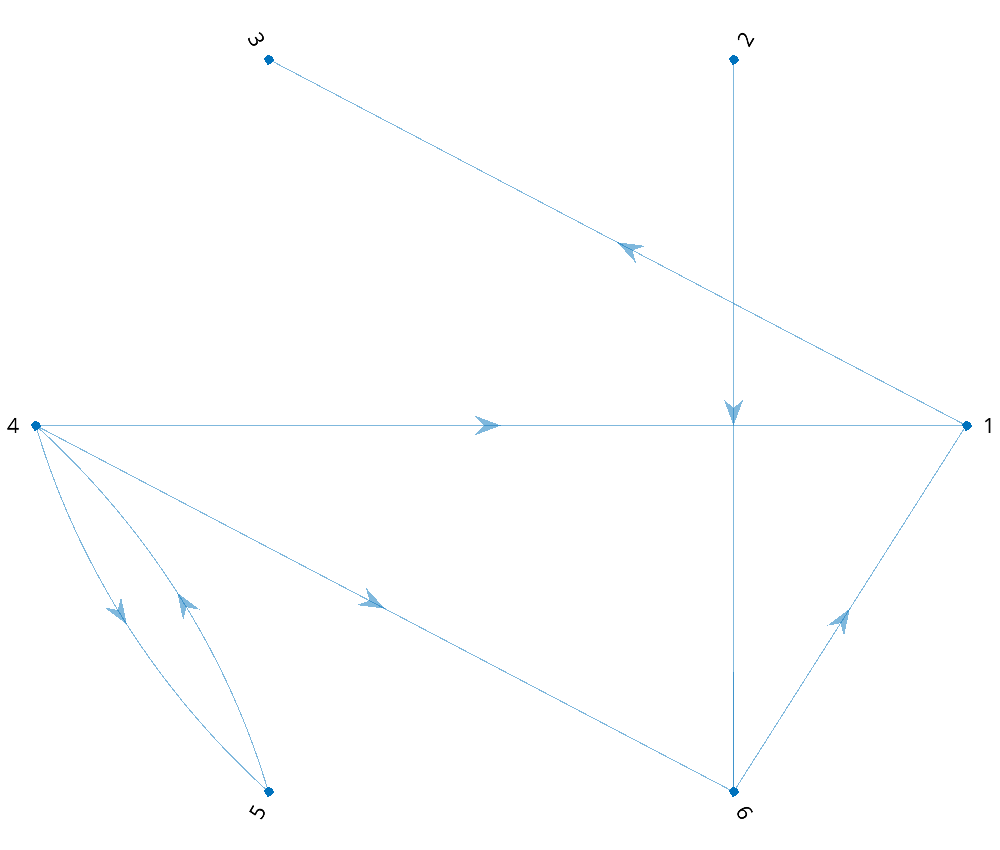
\includegraphics[scale=0.9]{../figures/A1_graph.png}
\end{center}

Vediamo quindi che le adiacenze fra nodi (pensando alla matrice, le dipendenze riga-colonna) sono:
\begin{table}[h!]
	\center \rowcolors{2}{white}{black!10}
	\begin{tabular} { c || c | c }
		\bfseries Nodo & \bfseries Raggiungibile & \bfseries Non raggiungibile \\
		\hline 
		1 & 1 3 & 2 4 5 6 \\
		2 & 1 2 3 6 & 4 5 \\
		3 & 3 & 1 2 4 5 6 \\
		4 & 1 3 4 5 6 & 2 \\
		5 & 1 3 4 5 6 & 2 \\
		6 & 1 3 6 & 2 4 5
	\end{tabular}
\end{table}

Notiamo che il nodo 6 ci fornisce la partizione migliore: $3 \times 3$ e $3 \times 3$.
Decidiamo quindi di prendere:
$$
\mathcal{P} = \{ 1, 3, 6 \}, \quad \mathcal{Q} = \{ 2, 4, 5 \}
$$
per cui la permutazione che manda $\mathcal{Q}$ in testa è:
$$
\Pi = \begin{pmatrix}
	0 & 1 & 0 & 0 & 0 & 0 \\
	0 & 0 & 0 & 1 & 0 & 0 \\
	0 & 0 & 0 & 0 & 1 & 0 \\
	1 & 0 & 0 & 0 & 0 & 0 \\
	0 & 0 & 1 & 0 & 0 & 0 \\
	0 & 0 & 0 & 0 & 0 & 1 \\
\end{pmatrix}
\begin{array}{c}
	2 \rightarrow 1 \\
	4 \rightarrow 2 \\
	5 \rightarrow 3 \\
	1 \rightarrow 4 \\
	3 \rightarrow 5 \\
	6 \rightarrow 6 \\
\end{array}
$$

Applicando $Pi A \Pi^T$ si ottiene quindi:
$$
\Pi A \Pi^T = \begin{pmatrix}
	A_{11} =
	\begin{pmatrix}
		0 &  0 &  0 \\
		0 &  0 & -1 \\
		0 & -1 &  0
	\end{pmatrix} &
	A_{12} = 
	\begin{pmatrix}
		0 &  0 &  3 \\
		3 &  0 & -2 \\
		0 &  0 &  0
	\end{pmatrix} \\
	0 &
	A_{21} = 
	\begin{pmatrix}
		0 &  1 &  0 \\
		0 &  0 &  0 \\
		1 &  0 &  0
	\end{pmatrix}
\end{pmatrix}
$$
che è una forma più agile per la risoluzione della matrice originale $A$.

Nella directory \lstinline|/matlab| si rende disponibile uno script \lstinline|block_decomp.m| per la decomposizione in matrici a blocchi come nell'esempio.
Un'esecuzione tipica dello script potrebbe avere l'aspetto:
\begin{lstlisting}[language=matlab, style=codestyle]	
p = block_decomp(A) % ottieni una permutazione
    Node      Reachable      Not reachable
    ____    _____________    _____________

     1      {[      1 3]}    {[  2 4 5 6]}
     2      {[  1 2 3 6]}    {[      4 5]}
     3      {[        3]}    {[1 2 4 5 6]}
     4      {[1 3 4 5 6]}    {[        2]}
     5      {[1 3 4 5 6]}    {[        2]}
     6      {[    1 3 6]}    {[    2 4 5]}
   
	 Choose an index: 6 % chiesto dallo script
>> A(p, p) % permuta A
\end{lstlisting}
da cui si ottiene la stessa matrice a blocchi riportata sopra.

\subsubsection{Riduzione iterata}
Ricordiamo di poter iterare ricorsivamente il processo di riduzione, cioè di poter trovare per ogni blocco $A_{ii}$ con $i \in \{ 1, 2 \}$ un $\Pi_i$ tale che:
$$
\Pi_i A_{ii} \Pi_i^T = \begin{pmatrix}
	A_{11}^{(i)} & A_{12}^{(i)} \\
	0 & A_{22}^{(i)} \\
\end{pmatrix}
$$
così che valga:
$$
\begin{pmatrix}
	\Pi_1 & 0 \\
	0 & \Pi_2
\end{pmatrix}
\begin{pmatrix}
	A_{11} & A_{12} \\
	0 & A_{22}
\end{pmatrix}
\begin{pmatrix}
	\Pi_1^T & 0 \\
	0 & \Pi_2^T
\end{pmatrix} =
\begin{pmatrix}
	\Pi_1 A_{11} \Pi_1^t & \Pi_1 A_{12} \Pi_2^T \\
	0 & \Pi_2 A_{22} \Pi_2^t \\
\end{pmatrix}
$$
$$
= \begin{pmatrix}
\begin{pmatrix}
	A_{11}^{(1)} & A_{12}^{(1)} \\
	0 & A_{22}^{(1)} \\
\end{pmatrix} & * \\
0 & 
\begin{pmatrix}
	A_{11}^{(2)} & A_{12}^{(2)} \\
	0 & A_{22}^{(2)} \\
\end{pmatrix}
\end{pmatrix}
$$
e via dicendo,
dove in $(*)$ comparrà qualcosa che al momento non ci interessa.

\subsubsection{Problemi agli autovalori per riduzione}
Notiamo che questo procedimento semplifica anche la risoluzione dei \textbf{problemi agli autovalori}: infatti iterando abbastanza, il problema si ridurrà a trovare i singoli autovalori di matrici sulla diagonale sempre più piccole, e quindi dal polinomio caratteristico di più facile risoluzione.

\subsection{Sistemi lineari}
Veniamo quindi alla trattazione dei sistemi lineari, che avevamo definito come forme $Ax = b$ con $A \in \mathbb{C}^{n \times n}, b \in \mathbb{C}^n$.

Studieremo 2 tipi di metodi risolutivi:
\begin{itemize}
	\item \textbf{Metodi diretti:} esatti ma dispendiosi, se eseguiti in aritmetica esatta (cioè senza arrotondamenti) poterebbero in un numero $n$ finito di passaggi alla soluzione esatta.
	Esempi di metodi diretti sono il \textbf{metodo di Cramer} (visto in 4.7.2) e l'\textbf{eliminazione di Gauss} (che vedremo fra poco);
	\item \textbf{Metodi iterativi:} meno accurati ma più efficienti computazionalmente, portano ad una successione $\{x_k\}_{k \in \mathbb{N}}$ di approssimazioni tali che $ \lim_{k \rightarrow +\infty} x_k = x$ soluzione esatta. Notiamo però che, in generale, è impossibile trovare il valore esatto di $x$ in un numero esatto di iterazioni. Per contropartita, risultano spesso molto più efficienti dei metodi diretti (esistono esempi di sistemi addirittura non risolvibili, nella pratica, con metodi diretti). 
\end{itemize}

\subsubsection{Sistemi triangolari}
Diamo la definizione parallela a quella di matrice triangolare:
\begin{definition}{Sistema triangolare}
	Si dice sistema triangolare un sistema della forma $Ux = c$ con $U$ matrice triangolare.
\end{definition}

Per un \textbf{sistema triangolare superiore}, si avrà la forma:
\[
\begin{cases}
    \begin{aligned}
			&& u_{11} x_1 + u_{12} x_2 + ... + u_{1,n-1} x_{n-1} + u_{1n} x_n = c_1 \\
			&&              u_{22} x_2 + ... + u_{2,n-1} x_{n-1} + u_{2n} x_n = c_2 \\
			&& \vdots \\
			&&                                 u_{n-1,n-1} x_{n-1} + u_{n-1,n} x_n = c_{n-1} \\
			&&                                                     u_{nn} x_n = c_n
		\end{aligned}
\end{cases}
\]

Il \textbf{metodo risolutivo} sarà allora la \textit{sostituzione all'indietro}, definita ricorsivamente come:
\[
	\begin{cases}
		x_n = \frac{c_n}{u_{nn}} \\\\ 
		x_i = \frac{ c_i - \sum_{j = i + 1}^n u_{ij} x_j }{u_{ii}}
	\end{cases}
\]
che equivale all'algoritmo, in MATLAB:
\lstinputlisting{../matlab/bck_subst.m}

Riguardo alla complessità, si potra dire che al passo $i$ si eseguono $n - i + n - i + 2 = 2(n - 1) + 2$ passaggi, cioè 2 per la divisione per $u_{jj}$ e la somma fra $c_i$ e il termine accumulato a destra, $n - i$ per i prodotti nella sommatoria e di nuovo $n - i$ per la sommatoria stessa.
Sarà allora che:
$$
\sum_{i = 1}^n \left( 2(n - i) + 2 \right) \sim O(n^2)
$$
cioè si ha complessità quadratica.

Osserviamo poi che per \textbf{sistemi triangolari inferiori} la situazione è uguale, cioè si risolve la prima equazione, si sostituisce il risultato nella seconda, e via dicendo:
\[
	\begin{cases}
		x_1 = \frac{c_1}{u_{11}} \\\\ 
		x_i = \frac{ c_i - \sum_{j = 1}^{i - 1} u_{ij} x_j }{u_{ii}}
	\end{cases}
\]
che equivale all'algoritmo, in MATLAB:
\lstinputlisting{../matlab/fwd_subst.m}

Il metodo ottenuto, speculare al quello di sostituzione all'indietro, viene detto \textit{sostituzione in avanti}, di costo identico ($O(n^2)$).

\subsubsection{Metodo di eliminazione di Gauss}
L'idea del metodo di eliminazione di Gauss è quella di partire da un sistema $Ax = b$, trasformarlo in un sistema equivalente $Ux = c$ (quindi triangolare superiore), ed applicare la sostituzione all'indietro.

Per arrivare alla forma $Ux = c$ si sostituiscono le equazioni del sistema con loro combinazioni lineari scelte in modo da annullare gli elementi inferiori alla diagonale.

L'idea è quella di eliminare, per ogni elemento $i$-esimo sulla diagonale a partire da quello in alto a destra, gli $n - i$ elementi che stanno al di sotto, cioè:

\begin{algorithm}
\caption{Eliminazione di Gauss}
\begin{algorithmic}
	\STATE \textbf{Input:} un sistema lineare qualsiasi $Ax = b$ % input
	\STATE \textbf{Output:} un sistema lineare triangolare superiore $Ux = c$ % output
	% body
	\FOR{$i = 1$ to $n$}
		\FOR{$j = i$ to $n$}
			\STATE Calcola il \textbf{moltiplicatore} $l_{ji} = \frac{a_{ji}^{(i - 1)}}{a_{ii}^{(i - 1)}}$
			\STATE Aggiungi alla riga $j$ la riga $i$ moltiplicata per $l_{ij}$
		\ENDFOR
	\ENDFOR
\end{algorithmic}
\end{algorithm}

Una semplice implementazione in MATLAB del suddetto algoritmo può essere la seguente:
\begin{lstlisting}[language=matlab, style=codestyle]	
function [A, b] = gauss_decomp(A, b)
    n = height(A);

    for i = 1:n % i itera sulle diagonali
        den = A(i, i);

        for j = (i + 1):n % j itera sulle righe
            mul = A(j, i) / den; % moltiplicatore
            
            A(j, :) = A(j, :) - A(i, :) * mul;
            b(j) = b(j) + b(i) * mul;
        end
    end
end
\end{lstlisting}
da cui si potrà ottenere una riduzione di Gauss semplicemente come:
\begin{lstlisting}[language=matlab, style=codestyle]	
	>> [U, c] = gauss_decomp(A, b)
\end{lstlisting}

\par\smallskip

Dal punto di vista della complessità, la riduzione in forma triangolare costa $O(\frac{2}{3}n^3)$, e chiaramente domina sul termine $O(n^2)$ della risoluzione di $Ux = c$ con la sostituzione all'indietro.

Facciamo una nota sulla fattibiltà della riduzione di Gauss, definendo:
\begin{definition}{Moltiplicatori di Gauss}
	I termini $l_{ji} = \frac{a_{ji}^{(i - 1)}}{a_{ii}^{(i - 1)}}$ vengono detti moltiplicatori.
\end{definition}
Chiaramente, per poter eseguire l'eliminazione di Gauss serve che $a_{jj^{j - 1}} \neq 0$ $\forall j = 1, ..., n - 1$.
Inoltre, i casi $a_{jj}^{j - 1} \approx 0$ possono causare problemi di instabilità numerica.
Vedremo in seguito metodi per ovviare a questo problema.

\subsubsection{Fattorizzazione LU}
Il primo passo dell'algoritmo di Gauss si può vedere come equivalente a moltiplicare l'equazione $Ax = b$ a sinistra per una particolare matrice $H_1$ triangolare inferiore:
$$
H_1 = \begin{pmatrix}
	1 & ... & ... & 0 \\
	-l_{21} & 1 & ... & 0 \\
	... \\ 
	-l_{n1} & ... & ... & 1
\end{pmatrix}
$$
con la diagonale a $1$ e i moltiplicatori sulla prima colonna, così che $A H_1$ risulti esattamente quello che volevamo per Gauss, cioè la combinazione lineare di ogni riga $j$ con l'prima riga moltiplicata per il moltiplicatore $l_{j1}$ (con $j > 2$).

Possiamo generalizzare questo processo a una serie di matrici $H_i$, per ogni elemento sulla diagonale, con la diagonale a $1$ e i moltiplicatori corrispondenti a $i$ sulla $i$-esima colonna:
$$
H_i = \begin{pmatrix}
	1 & ... & ... & 0 \\
	0 & 1 & ... & 0 \\
	... & -l_{ji} & ... & ... \\
	0 & -l_{ni} & ... & 1
\end{pmatrix}
$$
Così, ancora una volta, $A H_i$ risulterà quello che volevamo per Gauss, cioè la combinazione lineare di ogni riga $j$ con l'$i$-esima riga moltiplicata per il moltiplicatore $l_{ji}$.

Varrà allora he il metodo di Gauss sarà equivalente a considerare:
$$
H_{n - 1} H_{n - 2} \, ... \, H_1 A x = H_{n - 1} H_{n - 2} \, ... \, H_1 b
$$
e potremo quindi dire:
$$
H_{n - 1} H_{n - 2} \, ... \, H_1 A = U, \quad L = H_1^{-1} \, ... \, H_{n - 1}^1 
$$
da cui:
$$
A = LU
$$

Semplifichiamo i calcoli notando alcune proprietà delle matrici $H_j$:
\begin{enumerate}
	\item Hanno l'inversa facile, in quanto basta invertire i segni:
	$$
	H_i^{-1} = \begin{pmatrix}
		1 & ... & ... & 0 \\
		0 & 1 & ... & 0 \\
		... & l_{ji} & ... & ... \\
		0 & l_{ni} & ... & 1
	\end{pmatrix}
	$$

	\item Sono facili da moltiplicare, in quanto si può dire:
	$$
		H_{i_1} \cdot H_{i_2} = \begin{pmatrix}
		1 & ... & ... & 0 \\
		-l_{2i_1} & 1 & ... & 0 \\
		... & -l_{ji_2} & ... & ... \\
		-l_{ni_i} & -l_{ni_2} & ... & 1
	\end{pmatrix}
	$$
	e:	
	$$
	H_{i_1}^{-1} \cdot H_{i_2}^{-1} = \begin{pmatrix}
		1 & ... & ... & 0 \\
		l_{2i_1} & 1 & ... & 0 \\
		... & l_{ji_2} & ... & ... \\
		l_{ni_i} & l_{ni_2} & ... & 1
	\end{pmatrix}
	$$

	cioè semplicemente si somma sotto la diagonale.
\end{enumerate}

Questo significa che una volta svolta la prima parte dell'eliminazione di Gauss si è gia calcolata la fattorizzazione LU come la matrice dei moltiplicatori:
$$
H_{i_1}^{-1} \cdot H_{i_2}^{-1} = \begin{pmatrix}
	1 & ... & ... & 0 \\
	l_{21} & 1 & ... & 0 \\
	... & l_{3,2} & ...\\
	l_{n1} & l_{n2} & ... & 1
\end{pmatrix}
$$

\par\smallskip

Modifichiamo il codice MATLAB della scorsa sessione per calculare, oltre all'eliminazione di Gauss (cioè la matrice $U$), la matrice dei moltiplicatori $L$:

\lstinputlisting{../matlab/gauss_decomp.m}

A questo punto per calcolare la fattorizzazione LU di una matrice basterà eseguire:
\begin{lstlisting}[language=matlab, style=codestyle]	
>> [U, ~, L] = gauss_decomp(A, b)
>> L * U % idealmente dara' A
\end{lstlisting}
\par\smallskip

Si osserva quindi che se già si conoscono $L$ ed $U$ (magari di una matrice che dovremo usare spesso) risolvere $Ax = b$ costa $O(n^2)$, in quanto basta dire:
$$
Ax = b \, \Rightarrow \, LUx = b \implies x = U^{-1} L^{-1} b
$$
dove basta risolvere a cascata:
\[
	\begin{cases}
		Ly = b \\\
		Ux = y
	\end{cases}
\]
Questi sono due sistemi triangolari, uno \textbf{inferiore} (risolvibile per \textit{sostituzione in avanti}), l'altro \textbf{superiore} (risolvibile per \textit{sostituzione all'indietro}), da cui l'andamento complessivo $O(n^2)$.

In MATLAB, la soluzione si può quindi avere usando le funzioni definite finora:
\begin{lstlisting}[language=matlab, style=codestyle]	
>> [U, ~, L] = gauss_decomp(A, b)
>> y = fwd_subst(L, b)
>> x = bck_subst(U, y) % x e' la soluzione del sistema
\end{lstlisting}

Notiamo che questo vale se $L$ ed $U$ sono note (o come nell'esempio vengono calcolate), quindi tolto il prezzo dato dal doverle calcolare (come avevamo notato, conviene per matrici che magari dobbiamo usare spesso).

\subsubsection{Metodo di Gauss per variabili matriciali}
Se si vuole risolvere $AX = B$ con $X$ e $B$ matrici di vettori colonna di $s$ colonne:
$$
X = \begin{pmatrix}
	x_1 & ... & x_s
\end{pmatrix}, \quad
B = \begin{pmatrix}
	b_1 & ... & b_s
\end{pmatrix}
$$
cioè se si vogliono risolvere $s$ sistemi lineari con la stessa matrice $A$:
$$
Ax_1 = b_1, \quad ..., \quad Ax_s = b_s
$$
si può modificare l'algoritmo di Gauss, effettuando le mosse di Gauss sulla matrice aumentata $\begin{pmatrix}
	A \, | \, B
\end{pmatrix}$.
Alla fine troveremo una matrice $\begin{pmatrix}
	U \, | \, B^{(n - 1)}
\end{pmatrix}$, dove gli apici $(n - 1)$ rappresentano che è la $B$ che si ottiene all'$n-1$-esimo passaggio, che risolverà i sistemi triangolari superiori:
$$
Ux_1 = b_1^{(n - 1)}, \quad ..., \quad Ux_s = b_s^{(n - 1)}
$$

\subsubsection{Metodo di Gauss per il calcolo dell'inversa}
Un caso particolare è il \textbf{calcolo dell'inversa} con l'algoritmo di \textbf{Gauss-Jordan}.
Infatti, scegliendo:
$$
AX = I
$$
con $n = s$, le colonne in $X$ diventeranno l'inversa di $A$ (basti vedere che $A A^{-1} = I$ per definizione).

Facciamo un ultimo esempio, assistito da MATLAB, per comprendere a pieno questo risultato.
Vogliamo calcolare $A^{-1}$ come la soluzione del sistema $AX = I$, e capiamo quindi che quello che cerchiamo sono i vettori colonna $i_1, ..., i_n$ tali per cui:
$$
A i_1 = I_1, \quad ..., \quad A i_n = I_n
$$
con $I_i$ il vettore di zeri con un 1 all'$i$-esima riga.
Sfruttiamo allora l'eliminazione di Gauss per ricavare due matrici, $U$ e $B^{(n - 1)}$, tali che $Ux = B^{(n - 1)}$, con il vantaggio che $U$ è triangolare superiore e quindi risolvibile per sostituzione all'indietro.
Possiamo fare questo in MATLAB come:
\begin{lstlisting}[language=matlab, style=codestyle]	
AI = [A, eye(n)]
UB = gauss_decomp(AI, zeros(n, 1)) % argomento fittizio per b
U = UB(1:n, 1:n)
B = UB(1:n, (n + 1):(2 * n)
\end{lstlisting}

A questo punto potremo trovare le colonne $i_i$ come:
\begin{lstlisting}[language=matlab, style=codestyle]	
>> i1 = bck_subst(U, B(1:n, 1))
>> i2 = bck_subst(U, B(1:n, 2))
...
\end{lstlisting}
e infine concatenare le colonne come:
\begin{lstlisting}[language=matlab, style=codestyle]	
>> inv_A = [i1, ..., in]
\end{lstlisting}

In un unico script MATLAB, questo procedimento si realizza come:
\lstinputlisting{../matlab/gauss_inv.m}

\end{document}
